\documentclass[11pt,letterpaper]{article}
\usepackage[utf8]{inputenc}
\usepackage[T1]{fontenc}
\usepackage[spanish]{babel}
\usepackage{amsmath}
\usepackage{amsfonts}
\usepackage{amssymb}
\usepackage{graphicx}
\usepackage{lmodern}
\usepackage{xspace}
\usepackage{multicol}
\usepackage{hyperref}
\usepackage{float}
\usepackage{hyperref}
\usepackage{color}

\newcommand{\azul}[1]{\textcolor{MaterialBlue900}{#1}}
\usepackage{array}

\hypersetup{colorlinks=true,   linkcolor=MaterialBlue900}
%\usepackage[colorlinks=true, linkcolor=black, urlcolor=blue, pdfborder={0 0 0}]{hyperref}

\usepackage[left=2cm,right=2cm,top=2cm,bottom=2cm]{geometry}
\title{Modelos no paramétricos y de regresión 2018-1}
\author{Tarea examen: pruebas binomiales y tablas de contingencia}
\date{Fecha de entrega: 08/01/2017}
\setlength{\parindent}{0in}
\spanishdecimal{.}


\newcommand{\X}{\mathbb{X}}
\newcommand{\x}{\mathbf{x}}
\newcommand{\Y}{\mathbf{Y}}
\newcommand{\y}{\mathbf{y}}
\newcommand{\xbarn}{\bar{x}_n}
\newcommand{\ybarn}{\bar{y}_n}
\newcommand{\paren}[1]{\left( #1 \right)}
\newcommand{\llaves}[1]{\left\lbrace #1 \right\rbrace}
\newcommand{\barra}{\,\vert\,}
\newcommand{\mP}{\mathbb{P}}
\newcommand{\mE}{\mathbb{E}}
\newcommand{\mI}{\mathbf{I}}
\newcommand{\mJ}{\mathbf{J}}
\newcommand{\mX}{\mathbf{X}}
\newcommand{\mS}{\mathbf{S}}
\newcommand{\mA}{\mathbf{A}}
\newcommand{\unos}{\boldsymbol{1}}
\newcommand{\xbarnv}{\bar{\mathbf{x}}_n}
\newcommand{\abs}[1]{\left\vert #1 \right\vert}
\newcommand{\muv}{\boldsymbol{\mu}}
\newcommand{\mcov}{\boldsymbol{\Sigma}}
\newcommand{\vbet}{\boldsymbol{\beta}}
\newcommand{\veps}{\boldsymbol{\epsilon}}
\newcommand{\mC}{\mathbf{C}}
\newcommand{\ceros}{\boldsymbol{0}}
\newcommand{\mH}{\mathbf{H}}
\newcommand{\ve}{\mathbf{e}}
\newcommand{\avec}{\mathbf{a}}
\newcommand{\res}{\textbf{RESPUESTA}\\}
\newcommand{\rojo}[1]{\textcolor{MaterialRed900}{#1}}

\newcommand{\defi}[3]{\textbf{Definición:#3}}
\newcommand{\fin}{$\blacksquare.$}
\newcommand{\finf}{\blacksquare.}
\newcommand{\tr}{\text{tr}}
\begin{document}
\begin{table}[ht]
\centering
\begin{tabular}{c}
\textbf{Maestría en Computo Estadístico}\\
\textbf{Inferencia Estadística} \\
\textbf{Tarea 2}\\
\today \\
\emph{Enrique Santibáñez Cortés}\\
Repositorio de Git: \href{https://github.com/Enriquesec/Inferencia_Estad-stica/tree/master/Tareas/Tarea_2}{Tarea 2, IE}.
\end{tabular}
\end{table}

\begin{itemize}
\item[1.] Cuando una máquina no se ajusta adecuadamente tiene una probabilidad 0.15 de producir un artículo defectuoso. Diariamente, la máquina trabaja hasta que se producen 3 artículos defectuosos. Se detiene la máquina y se revisa para ajustarla. ¿Cuál es la probabilidad de que una máquina mal ajustada produzca 5 o más artículos antes de que sea detenida? ¿Cuál es el número promedio de artículos que la máquina producirá antes de ser detenida?

\res
Sea $X$ el número de artículos producidos antes de que se produzcan 3 artículos defectuosos, entonces podemos decir que $X\sim BN(3,0.15).$ Por lo tanto, \textbf{la probabilidad de que una máquina mal ajustada produzca 5 o más artículos antes de que sea detenida} es (ocupamos la función en R pnbinom(1, 3, 0.15)):
$$\mP(X\geq 5) =1-\mP(X\leq 4)=1-\sum_{x=3}^4{x-1 \choose 3-1}(1-0.15)^{x-3}(0.15)^3= 1-0.01198125=0.9880187.$$
Por como se distribuye $X$ podemos decir que \textbf{el número promedio de artículos que la máquina producirá antes de ser detenida} es
$$\mE(X)=\frac{r}{p}=\frac{3}{0.15}=20. \finf$$

\item[2.] Los empleados de una compañía de aislantes son sometidos a pruebas para detectar residuos de asbesto en sus pulmones. Se le ha pedido a la compañía que envíe a tres empleados, cuyas pruebas resulten positivas, a un centro médico para realizarles más análisis. Si se sospecha que el 40 \% de los empleados tienen residuos de asbesto en sus pulmones, encuentre la probabilidad de que deban ser analizados 10 trabajadores para poder encontrar a 3 con resultado positivo.

\res
Sea $Y$ el número de trabajadores que se realizan las pruebas hasta encontrar 3 empleados con resultados positivos. Y como la probabilidad de que algún empleado tenga residuos de asbesto en sus pulmones (dar positivo en la pruebas) es de $0.40$. Entonces podemos concluir que $Y\sim BN(3,0.4).$ Por lo que la \textbf{probabilidad de que deban analizar 10 trabajadores para encontrar a 3 con resultado positivo es} (ocupamos la función en dnbinom(10, 3, 0.40) en R):
$$\mP(Y=10) = {10-1 \choose 3-1}(1-0.40)^{10-3}(0.40)^3= 0.06449725\ \ \ \ \finf$$

\item[5.] Considera $X$ una v.a. con función de distribución $F$ y función de densidad $f$, y sea $A$ un intervalo de la línea real $\mathbb{R}$. Definamos la función indicadora $1_{A}(x):$
\begin{equation*}
1_{A}(x) = \left\{\begin{array}{ccr}
1 & \text{si} \ x\in A\\
0 & \text{en otro caso}
\end{array}\right.
\end{equation*}
Sea $Y=1_{A}(x).$ Encuentre una expresión para la distribución acumulada y el valor esperado de $Y$. 
\res 
Consideremos dos casos:\\
cuando $X$ es discreta tenemos que la función de densidad es 

$$f(Y=y)=\mP(1_{A}(x)=y)=\mP(\{x:1_{A}(x)=y\}).$$
\begin{equation*}
f(y)=\left\{ \begin{array}{cc}
\mP(x\in A) & \text{para y=1}\\
\mP(x\not \in A) & \text{para y=0}\\
0 & \text{en otro caso}
\end{array}\right.
\end{equation*}
El valor esperado es
$$\mE[Y]=\sum y f(y)=1\cdot f(1)+0\cdot f(0)=1\cdot f(1)=\mP(x\in A)\ \ \ \finf$$

\item[6.] Las calificaciones de un estudiante de primer semestre en un examen de química se describen
por la densidad de probabilidad
$$f_y(y)=6y(1-y)\ \ \ \ 0\leq y \leq 1,$$
donde $y$ representa la proporción de preguntas que el estudiante contesta correctamente. Cualquier calificación menor a 0.4 es reprobatoria. Responda lo siguiente:
\begin{itemize}
\item[a)] ¿Cuál es la probabilidad de que un estudiante repruebe?
\item[b)] Si 6 estudiantes toman el examen, ¿cuál es la probabilidad de exactamente 2 reprueben?
\end{itemize}
\res
Por como esta definida la función de probabilidad podemos decir que $Y$ es es una variable continua. Ahora, solo para comprobación veamos que realmente sea una función de probabilidad, para ello observemos que
$$\int_{-\infty}^\infty f_y(y)=\int_{0}^1 6y(1-y)=3y^2-2y^3|_0^1=1.$$
Por lo tanto observamos que si es una función de probabilidad. 

Entonces \textbf{la probabilidad de que un estudiante repruebe es}
$$f_y(Y<0.4)=\int_0^{0.4}f_y(y)=\int_0^{0.4} 6y(1-y)=3y^2-2y^3|_0^{0.4}=0.352 $$
Ahora, sea $X$ el número de estudiantes de reprueban el examen de un conjunto de 6 estudiantes que realizaron el examen. Por definición podemos decir que $X\sim Bin(6,p)$ donde $p$ es la probabilidad de reprobar, pero si consideramos que las calificaiones de los estudiantes se distribuye como la variable $Y$, entonces podemos concluir que $X\sim Bin(6,0.352).$  Por lo tanto, \textbf{la probabilidad de que exactamente 2 estudiantes reprueben es} (usamos la función dbinom(x=4, size = 6, prob = 0.325):
$$\mP(X=2)={6\choose 2}0.325^2(1-0.325)^4 =0.328907 \ \ \ \finf$$

\item[8.] En una oficina de correo los paquetes llegan según un proceso de Poisson de intensidad $\lambda$. Hay un costo de almacenamiento de $c$ pesos por paquete y por unidad de tiempo. Los paquetes se acumulan en el local y se despachan en grupos cada $T$ unidades de tiempo (es decir, se despachan en $T , 2T , 3T , \cdots)$. Hay un costo por despacho fijo de $K$ pesos (es decir, el costo es independiente del número de paquetes que se despachen). (a) ¿Cuál es el costo promedio por paquete por almacenamiento en el primer ciclo $[0, T ]$? (b) ¿Cuál es el costo promedio por paquete por almacenamiento y despacho en el primer ciclo? (c) ¿Cuál es el valor de $T$ que minimiza este costo promedio?

\res 
Sea X el número de paquetes que llegan al correo en un intervalo de tiempo $T$, este se distribuye como un proceso Poisson con intensidad $\lambda$. Entonces el costo total promedio por almacenamiento es: 
$$\mE[C]=\mE[X\cdot c \cdot T]=cT\mE[X]=cT\cdot (\lambda T)=cT^2\lambda.$$
Y ahora el número esperado de paquetes en el primer ciclo es: 
$$\mE[X]=\lambda T.$$

Por lo que, \textbf{(a) el costo promedio por paquete por almacenamiento es:}
$$\frac{cT^2\lambda}{\lambda T}=cT.$$

Ahora sea $G$ el costo total de almacenamiento y despacho para el primer ciclo $[0,T]$ definido como
$$G=cXT+K.$$
Entonces el costo promedio total por almacenamiento y despacho es
$$\mE[G]=\mE[cXT+K]=cT^2\lambda+K.$$

Lo anterior implica que \textbf{el costo promedio por paquete por almacenamiento y despacho en el primer ciclo} es:
$$\bar{\mE[G]}=\frac{cT^2\lambda+K}{\lambda T}.$$

Utilizando el resultado anterior, diferenciamos e igualamos a cero para encontrar el mínimo.
$$\bar{\mE'[G]}=c-\frac{K}{\lambda T^2}$$
Igualamos a cero:
\begin{equation*}
\begin{array}{ccc}
c-\frac{K}{\lambda T^2} &=& 0\\
&&\\
T^2&=&\frac{K}{c\lambda}\\
&&\\
T&=&\sqrt{\frac{K}{c\lambda}}.
\end{array}
\end{equation*}
Usando el criterio de segunda derivada para determinar si es un máximo o minino:
$$\bar{\mE''[G]}=2\frac{K}{\lambda T^3}.$$
Evaluando la segunda derivada en $T=\sqrt{\frac{K}{c\lambda}}$, observamos que $\bar{\mE''[G]}>0$, por lo que podemos concluir que es un mínimo. En conclusión, \textbf{el valor de $T$ para el cuál minimiza el costo promedio por paquete por almacenamiento y despacho en el primer ciclo es} $\sqrt{\frac{K}{c\lambda}}\ \ \ \finf$
\item[9.] Considere la siguiente función
\begin{equation*}
F(x)=\left\{ \begin{array}{cl}
0 & \text{para} \ x<0\\
0.1 & \text{para} \ x=0\\
0.1+0.8x & \text{para} \ 0<x<3/4\\
1 & \text{para } 3/4\leq x
\end{array} \right.
\end{equation*}
¿Es una función de distribución? Si es una función de distribución, ¿corresponde a una variable
aleatoria discreta o continua?

\res 
Observemos por como esta definida la función tenemos que $0\leq F(x) \leq 1$. Y además $\lim_{x\rightarrow\infty^-}F(x)=0$ y $\lim_{x\rightarrow\infty^+}F(x)=1$. Por lo que podemos concluir que $F(x)$ si es una función de distribución. Ahora, observemos que la función esta definida para $x=0$ y $x=3/4$, si $X$ fuera una $X$ fuera una variable continua, por definición $F(x=a)=0,$ por lo que $X$ es discreta en $x=0$ y $x=3/4$. Y como $F(x)$ es continua en $0<x<3/4$ podemos decir que $X$ es continua en ese intervalo. Entonces como $X$ es continua y discreta para ciertos valores, decimos que $X$ es "mixta". Esto igual se puede mostrar observando la grafica de la función $F(X) \ \ \ \ \finf$
\begin{figure}[H]
\centering
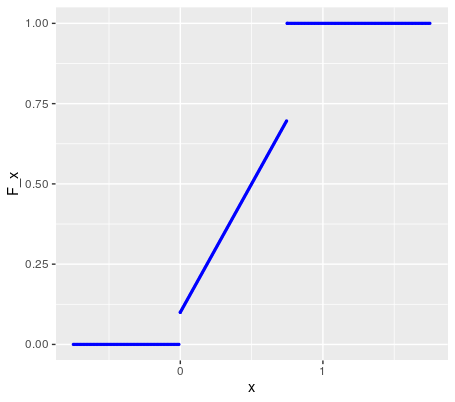
\includegraphics[scale=0.7]{ejercicio_9.png}
\caption{Función de densidad mixta.}
\end{figure}

\end{itemize}


\textbf{Honour problems (no es obligatorio entregarlos, pero dan crédito extra)}\\

\begin{itemize}
\item[1.] Cambiando las hipótesis 2 y 3 que se usaron para contruir los procesos de Poisson homogéneos
a la forma indicada en la diapositiva 135, deduzca la distribución del número de eventos que
ocurren durante el intervalo $[t_1 , t_2]$.

\item[2.] Sea $N(t), \ t\leq 0$ un proceso de Poisson con parámetro $\lambda >0$. Para $0<\mu <t$ y $0\geq k\geq n,$ calcule la probabilidad $P(N(u)=k|N(y)=n)).$ Interpreta los resultados.
\end{itemize}

\textbf{Ejercicios de las notas. }
\begin{itemize}

\item Distribución uniforme continua.
\begin{itemize}
\item[i)] Crea una columna con 100 valores de una $Unif(0,1)$ en el software de tu preferencia.
\item[ii)] Construye otra columna con la fórmula $$x=-2\log(1-y).$$
\item[iii)] Construye el histograma de esta nueva columna y concluye.
\end{itemize} 

\item El modelo Normal o Gaussiano. Se han realizado ciertas pruebas de resistencia en ladrillos obteniéndose las mediciones que a continuación se muestran, agrupadas en una tabla de frecuencias.
\begin{table}[H]
\centering
\begin{tabular}{ccccc}
\hline
Interv. & De & Hasta & Frecuencia & Frec. relativa\\ \hline
1 & 28.70 & 31.65 & 5 & 5.56\\
2 & 32.65 & 36.60 & 6 & 6.67\\
3 & 36.60 & 40.55 &11 & 12.22\\
\hline
\end{tabular}
\end{table}
\begin{itemize}
\item[a)] Traza el histograma.
\item[b)] Calcula la probabilidad de cada intervalo de clase de la tabla de frecuencias asumiendo que las resistencias siguen una distribución normal con media 45.47 y varianza 58.19.
\item[c)] Compara las frecuencias relativas con lasa probabilidades bajo normalidad ¿Qué se puede concluir? Esta es la idea base de una prueba de Bondad de Ajuste conocida como $\chi^2$ de Pearson. Si la media y la varianza de la normal no se conocen de antemano, podemos usar los valores muestrales correspondientes como una aproximación de los mismos. A esto lo llamamos estimación de parámetros y ya hablaremos más adelante de las cualidades de los estimadores.
\end{itemize}

\item El modelo exponencial. Consideremos un sistema formado por 5 componentes idénticos conectados en serie tal como se muestra a continuación:

Tan pronto como un componente falla, el sistema completa falla. Supongamos que cada componente sigue un modelo de tiempo a la falla exponencial con $\theta=100,$ y que los componentes fallan en forma independiente una de la otra. Definamos los eventos
$$A_i=\{i-\text{ésimo componente dura al menors t horas}\}\ i=1,2,3,4,5. $$
Las $A_i's$ son independientes e identicamente distriuidas. Sea $X$ el tiempo de la falla del sistema.
\begin{itemize}
\item[a)] El evento $\{ X\geq t\}$, ¿a cuál evento, en términos de las $A_i's$ es equivalente?
\item[b)] Usando la independencia de las $A_i's$ calcula $\mP\{ X\geq t\}$. Obtén $F(t)=\mP(X\leq t).$ ¿Cuál es la distribución de $X$?
\item[c)] Si en lugar de 5 componenetes tenemos $n$, ¿cuál es la distribución de $X$?
\end{itemize}

\item El modelo Weibull. 
\begin{enumerate}
\item Gráficar la función Weibull para los siguientes valores de los parámetros 

Algebraicamente, o bien generando variables con ésta distribución y construyendo un histograma.


\item Gráfica las funciones de confiabilidad y riesgo para cada uno de los casos anteriores.

\item Si $h(t)= a+bt$, ¿cuál es la densidad asociada?

\item Estudiar las funciones de riesgo para la distribución Normal, Gamma y Lognormal. ¿Cuál es la principal dificultad en estos casos?
\end{enumerate}
\item El modelo Beta. En el ejemplo 


\item Resumiendo, tenemos que el modelo normal y el modelo Weibull producen los siguientes momentos: 

¿Qué distribución debería un estadístico recomendar según la evidencia? ¿Por qué?
\end{itemize}
\end{document}